\documentclass{article}
\usepackage[12pt]{extsizes}
\usepackage{cmap}
\usepackage[utf8]{inputenc}
%\usepackage[cp1251]{inputenc}
\usepackage[T2A]{fontenc}
\usepackage[russian]{babel}
\usepackage{color}
\usepackage{hyperref}
\usepackage{enumerate}
\usepackage{amsmath,amssymb, wasysym}
\numberwithin{equation}{section}
\makeatletter
\@addtoreset{equation}{section}
\makeatother
%\usepackage{chngcntr}
%\counterwithin{equation}{section}
\usepackage{enumitem}
\usepackage{epstopdf}
\usepackage{graphicx}
\usepackage[warn]{mathtext} 

%\graphicspath{{noiseimages/}}
\hypersetup{unicode = true, colorlinks, citecolor = red, filecolor = red, linkcolor = blue, urlcolor = blue }

\usepackage[left=2cm,right=2cm,
    top=2cm,bottom=2cm,bindingoffset=0cm]{geometry}
    
    \RequirePackage{caption2} 
\renewcommand\captionlabeldelim{ -} 

\begin{document}

\def\figurename{Рисунок}



\pagestyle{empty}
\begin{center}

{\LARGE\bf{Мануал. Программа NeiSys}}\par
\Large{Трофимов Е.П.}

\end{center}

 %\par \par *Конспект написан с целью 
\newpage



\setcounter{tocdepth}{2}  %numiric of pages
\tableofcontents


\newpage




%%%%%%%%%%%%%%%%%%%%%%%%%%%%%%%%%%%%%%%%%%%%%%%%%%%%%%%%%%%%%%%%%%%%%%%%%%%%%%%%%%%%%%%%%%%%%%%%%%%%%%%%%%%%%%%%%%%%%%%%%%%%%%%%%%%%%%%
\section{Практическое руководство}
%%%%%%%%%%%%%%%%%%%%%%%%%%%%%%%%%%%%%%%%%%%%%%%%%%%%%%%%%%%%%%%%%%%%%%%%%%%%%%%%%%%%%%%%%%%%%%%%%%%%%%%%%%%%%%%%%%%%%%%%%%%%%%%%%%%%%%%
\subsection{Запуск}


\qquad Для установки необходимо установить JVM (Java Virtual Mashine). Для этого заходим на \href{https://java.com/ru/download/manual.jsp}{официальный сайт Java}, скачиваем версию, соотвутствующую нашей операционной системе, устанавливаем и перезагружаем компьютер. 



После этого можно запускать программу - открываем файл {\bf NeiSys.jar}. После запуска должно появиться следующее окно:

\begin{figure}[h]
\center{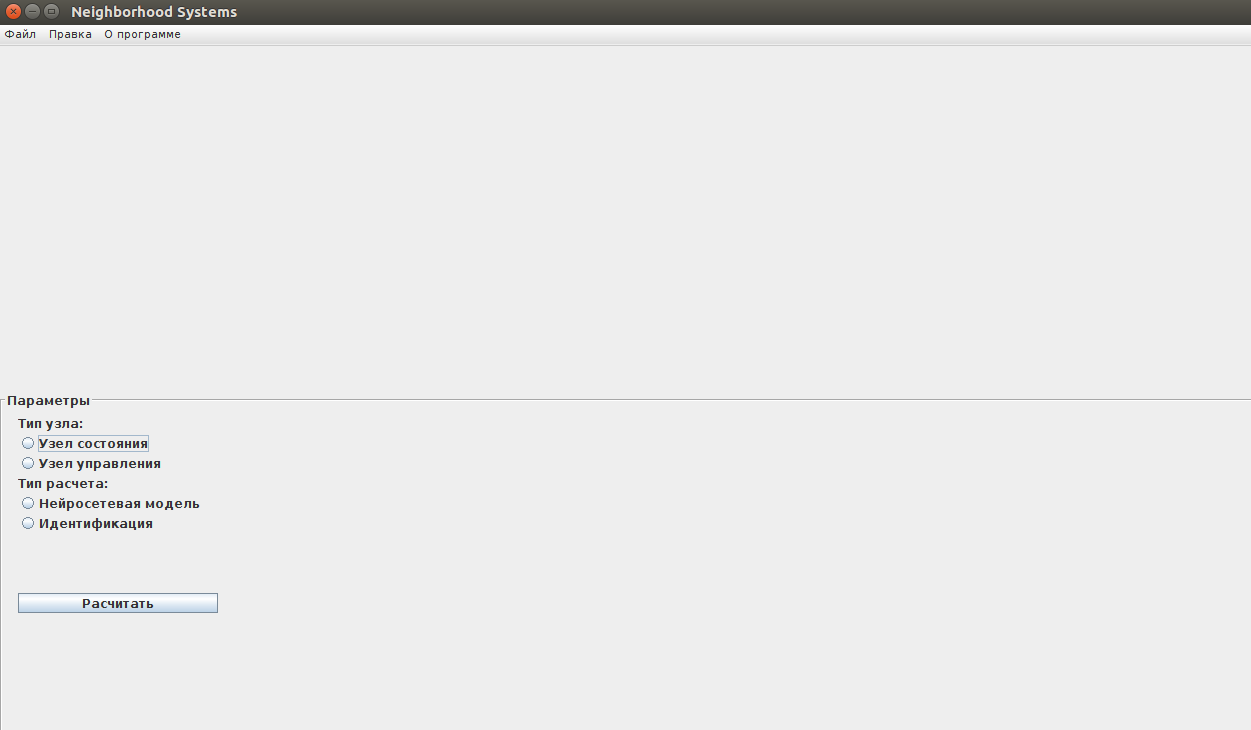
\includegraphics[width=0.6\linewidth]{pic/start.png}}
\caption{Стартовая панель программы.}
\label{ris:image}
\end{figure}



Если же данное окно не появилось, вероятнее всего что-то пошло не так при установке Java. Проверьте еще, правильно ли прошла установка. Возможно понадобиться прописать переменную JAVA\_HOME (возможные ошибки при установке Java не такая уж редкость, поэтому решение большинства из них можно прогуглить, например, \href{https://www.java.com/ru/download/help/path.xml}{настройка системной переменной}).

\subsection{Описание простейшего функционала}
\qquad Данная программа предназначена для \textcolor{red}{для работы с окрестностными системами, параметры (узлов и связей) которых являются скаляры, векторы и матрицы.}

Алгоритм программы следующий: начиная с первого узла в направлении связей просчитывает параметры узлов, и для узлов конечных узлов состояния (State) считает выходной вектор. Конечными мы называем те состояний, которые не имеют выходящие связи. При этом на узел могут оказывать воздействие не только узлы, от которых идет связь, но входящий узел (правая кнопка мыши -> Задать входящий вектор).

{\textbf{ Если у какого-либо узла параметры отсутствуют, то в процессе расчета программа должна автоматические решить задачу идентификации для этого узла.}}


\begin{figure}[h]
\center{\includegraphics[width=0.8\linewidth]{pic/comm.png}}
\caption{Общий вид.}
\label{ris:image2}
\end{figure}


Программа позволяет выполнять простейшие арифмитические операции над скалярами и матрицами.

\subsection{Общие правила} 

	\qquad При соединении связи между двумя узлами: параметры узла из которого выходят перемножаются на параметры связи и воздействуют на второй узел в зависимости от типа связи: сложением или умножением.

	
Рассмотрим пример. Пусть имеется два связанных узла:
	
	\begin{figure}[h]
\center{\includegraphics[width=0.3\linewidth]{pic/ex1.png}}
\caption{Общий вид.}
\label{ris:image3}
\end{figure}
	
	
Параметры всех частей системы -- скаляры и равны $2$. 	Тогда, если тип связи аддитивный "a", то получим:
$$
Out = P(Control2) * P(R) + P(State1) = 2 * 2 + 2 = 6.
$$
 
 \begin{figure}[h]
\center{\includegraphics[width=0.4\linewidth]{pic/ans1.png}}
%\caption{Общее правило перемножения узла на параметр.}
\label{ris:image4}
\end{figure}
	
Если же тип связи "m" (мультипликативный), тогда
$$
Out = P(Control2) * P(R) * P(State1) = 2 * 2 * 2 = 8.
$$ 
 \begin{figure}[h]
\center{\includegraphics[width=0.4\linewidth]{pic/ans2.png}}
%\caption{Общее правило перемножения узла на параметр.}
\label{ris:image5}
\end{figure}	


\newpage
При этом, если узел имеет несколько входящих связей, то исходящий вектор получается путем суммирования всех входящих параметров. Для примера, добавим к предыдущему случаю еще один узел.

\begin{figure}[h]
\center{\includegraphics[width=0.4\linewidth]{pic/ex2.png}}
\caption{Случай нескольких входящих связей.}
\label{ris:image6}
\end{figure}


Здесь параметр узла State7 равен $3$, а параметр его выходящий связи равен $1$. Тогда, выходящим вектором для State1 получим: 
$$
Out = \left[ P(Control2) * P(R_{Control2}) * P(State1)\right] + \left[P(State7) * P(R_{State7}) + P(State1)\right]=$$ $$  = [2 * 2 * 2] + [3 *1 + 2] = 8 + 5 = 13.
$$ 

\begin{figure}[h]
\center{\includegraphics[width=0.4\linewidth]{pic/ans3.png}}
%\caption{Случай нескольких входящих связей.}
\label{ris:image7}
\end{figure}


\qquad 

\newpage
\subsection{Операции с числами}


\qquad Особенности данной программы позволяют выполнять простейшие арифмитические действия над числами: сложение, умножение и деление.

\subsubsection{Сложение двух чисел}

\qquad Для того, чтобы сложить два числа нужно добавить на панель два узла, тип связи выбрать аддитивным и параметром связи указать равным $1$.
Пример:

\begin{figure}[h]
\center{\includegraphics[width=0.4\linewidth]{pic/ex3.png}}
\caption{Сложение двух чисел.}
\label{ris:image8}
\end{figure}


Здесь $P(State9) = 3, \ P(R) = 1, P(State8) = 2.$
Тогда получим:
$$
P(State9) * P(R) + P(State8) = 2 * 1 + 3 = 5.
$$
\begin{figure}[h]
\center{\includegraphics[width=0.4\linewidth]{pic/ans4.png}}
\caption{Сложение двух чисел.}
\label{ris:image9}
\end{figure}

\subsubsection{Умножение двух чисел}

\qquad Для того, чтобы умножить два числа нужно выполнить все действия как и для сложения, только вместо аддитивной связи выбрать мультипликативую. Тогда пример выше даст следующее:
$$
P(State9) * P(R) * P(State8) = 2 * 1 * 3 = 6.
$$
\begin{figure}[h]
\center{\includegraphics[width=0.4\linewidth]{pic/ans4.png}}
\caption{Умножение двух чисел.}
\label{ris:image10}
\end{figure}
 \newpage

\subsubsection{Деление двух чисел}

\qquad Деление двух чисел в данной программе отличается от сложения и умножения. Здесь деление реализовано через решение уравнения $ax = b$. Для того, чтобы найти $b/a$ нужно добавить всего один узел. И задать для него не параметры, а входящий вектор $a$ и исходящий вектор $b$. При этом на экране у узлса должны появиться параметры "I" и "O" с указанием размерности вектором. 

\begin{figure}[h]
\center{\includegraphics[width=0.2\linewidth]{pic/ex4.png}}
\caption{Деление двух чисел.}
\label{ris:image11}
\end{figure}

Далее тип расчета отмечаем "Идентификация" и нажимаем "Расчитать". В качества примера возьмем входящий вектор равным $3$, а исходящий -- $6$. В результате расчета:
\begin{figure}[h]
\center{\includegraphics[width=0.4\linewidth]{pic/ans6.png}}
\caption{Деление двух чисел.}
\label{ris:image12}
\end{figure}





\subsection{Действия с матрицами}

\qquad В данной программе действия с матрицами аналогичны действиям с числами. Единственное, что стоит упомянуть отдельно, что в случае задачи идентификации узел будет выдавать матрицу перехода в евклидовом базисе в векторном случае и псевдообратную в матричном. 

\newpage

\section{Руководство для программистов}

\subsection{Структура программы}
UML-диграмма:

\begin{figure}[h]
\center{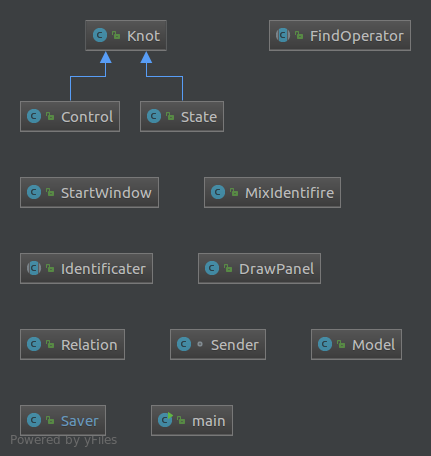
\includegraphics[width=0.3\linewidth]{pic/umlDiag.png}}
\caption{UML-диаграмма.}
\label{ris:image}
\end{figure}



\end{document}
\grid
\grid
\grid
\grid
